% Write-up plan for the whole GT2027 paper: figure, table and equation lists, then one section per paper
% section (subsection headings, content, figures, tables, equations and their purpose).
% Build: bash build_plan.sh (pdflatex twice; --figs also redraws the figures).
% Paper figures are read from ASME_2027/figures/, each drawn by figures/code/<same name>.py.
\documentclass[10pt]{article}
\usepackage[utf8]{inputenc}
\usepackage[T1]{fontenc}
\usepackage{lmodern}
\usepackage{textcomp}
\usepackage[a4paper,margin=18mm]{geometry}
\usepackage{amsmath,amssymb,bm}
\usepackage{booktabs,float,graphicx,array,enumitem,tabularx}
\usepackage[dvipsnames]{xcolor}
\usepackage[colorlinks=true,linkcolor=MidnightBlue,urlcolor=MidnightBlue]{hyperref}
\setlength{\parskip}{4pt}
\setlength{\parindent}{0pt}
\setlist{itemsep=1pt,topsep=2pt}
\setlength{\emergencystretch}{2em}
\newcommand{\um}{\textmu m}
\graphicspath{{../figures/}}
\newcommand{\st}[1]{\textsf{\small[#1]}}
\newcommand{\deta}{\Delta_{\mathrm{mesh}}/\eta_{K,193}}
% candidate paper figure: file in ../figures, width fraction, caption; a box if the file is not drawn yet
\newcommand{\planfig}[3]{\begin{figure}[H]\centering
  \IfFileExists{../figures/#1}{\includegraphics[width=#2\textwidth]{#1}}{\fbox{\parbox{0.6\textwidth}{\centering
  \texttt{\detokenize{#1}}: not drawn yet}}}\caption{#3}\end{figure}}

\title{GT2027 paper: write-up plan}
\author{24 November 2026}
\date{}

\begin{document}
\maketitle
\vspace{-8mm}

The plan for the whole paper, section by section: subsection headings, content, and the figures, tables and
equations with their purpose. Sections planned so far: 1 Introduction, 2 Research Aims, 3 Methods, 4.1 and 4.2 of the Results. Each agreed section is
written into \texttt{manuscript/main\_claude.tex}. Figures are in \texttt{ASME\_2027/figures/}, each drawn by the
script of the same name in \texttt{figures/code/}.

\section*{Figures, tables and equations}

Status: \st{exists} usable as it is; \st{rework} content right, data or layout to be updated; \st{new} not yet
made; \st{draft} made for this plan, to be finalised; \st{interim} drawn from the data available now.

\textbf{Figures}, in the order they appear in the paper.\par
{\centering\footnotesize
\begin{tabularx}{\textwidth}{@{}l l X l l@{}}
\toprule
ID & section & content & script (\texttt{figures/code/}) & status \\
\midrule
F1 & 1 & transition mechanism on the HPT suction surface against $\mathrm{Re}_x$; Fig.~1 of Kar et al.\ (2026), from Clark et al.\ (2024), reused & \texttt{fig\_transition\_map.py} & exists \\
F2 & 3.1 & (a) domain, boundary conditions, regions above the plate; (b) hole regions & \texttt{fig\_config\_regions.py} & draft \\
F3 & 3.2 & 13 line classes, plate and centre plane & \texttt{fig\_mesh\_classes.py} & draft \\
F4 & 3.3 & volume fraction above $\deta$, per region, 5 meshes & \texttt{fig\_resolution.py} & interim \\
F5 & 4.1 & static pressure and reversed fraction along the hole, six rungs & \texttt{fig\_hole\_axis.py} & rework \\
F6 & 4.1 & mean axial velocity in the diffuser, centre plane and section $s/D=-1.1$ & \texttt{fig\_diffuser\_flow.py} & rework \\
F7 & 4.1 & motion of the diffuser bubble: volume traces, spectra, coherence with BR & \texttt{fig\_bubble\_motion.py} & interim \\
F8 & 4.1 & plan view of near-wall $k/U_\infty^2$ and $\gamma$ & \texttt{fig\_wall\_state.py} & rework \\
F9 & 4.1 & spot growth and merger: space--time diagram, snapshot sequence & \texttt{fig\_spots.py} & new \\
F10 & 4.1 & $H$ and $C_f$ along the plate, centreline and mid-pitch & \texttt{fig\_bl\_params.py} & new \\
F11 & 4.1 & profiles of $U$, $k$, $\gamma$ at $x/D=10$ & \texttt{fig\_bl\_profiles.py} & rework \\
F12 & 4.1 & $\bar\eta$, centreline and mid-pitch $\eta$ against $x/D$, with data & \texttt{fig\_eta\_x.py} & rework \\
F13 & 4.1 & $\eta$ on the wall & \texttt{fig\_eta\_wall.py} & new \\
F14 & 4.1 & classic $\Pr_t$ of the reference, centre plane and $x/D=10$ & \texttt{fig\_prt\_classic.py} & new \\
F15 & 4.2 & RANS 50M $\ln\mu_t$ split into energy, length, alignment, against the 193M & \texttt{fig\_meff\_split.py} & rework \\
F16 & 4.2 & classic regional $\Pr_t$ of the 193M against 0.9 and the literature & \texttt{fig\_prt\_regions.py} & new \\
F17 & 4.2 & $k/U_\infty^2$ and $L_{\mathrm{eff}}/D$ on cross-planes $x/D$ 4, 10, 20 & \texttt{fig\_cross\_planes.py} & new \\
F18 & 4.2 & length ratio and alignment on the centre plane & \texttt{fig\_centre\_factors.py} & rework \\
F19 & 4.2 & $P_k$, $\varepsilon$ and lengths along wall-normal lines & \texttt{fig\_budget\_lines.py} & new \\
F20 & 4.2 & spanwise diffusion: directional ratios against the data, lateral flux deficit & \texttt{fig\_prt\_data.py} & rework \\
\bottomrule
\end{tabularx}\par}

\textbf{Tables}, in the order they appear in the paper.\par
{\centering\footnotesize
\begin{tabularx}{\textwidth}{@{}l l X l l@{}}
\toprule
ID & section & content & source & status \\
\midrule
T1 & 3.1 & rungs and meshes: $s$, cells, solver, model, filter, BR, averaging & mesh files, \texttt{hole\_discharge} & draft \\
\bottomrule
\end{tabularx}\par}

\textbf{Equations}, in the order they are numbered in the paper.\par
{\centering\footnotesize
\begin{tabular}{@{}l l l l@{}}
\toprule
ID & section & quantity & in the draft \\
\midrule
E1 & 1 & Boussinesq eddy-viscosity relation & new \\
E2 & 1 & gradient-diffusion hypothesis for the turbulent heat flux, $\Pr_t$ & new \\
E3 & 3.1 & $\mathrm{Re}_D$, $\theta$ & numbered (\texttt{eq:re}) \\
E4 & 3.1 & BR, DR, VR, $I$ & numbered (\texttt{eq:br}) \\
E5 & 3.1 & adiabatic effectiveness $\eta$, pitch average $\bar\eta$ & inline; numbered in the paper \\
E6 & 3.2 & point count per class, $N(s)$ & numbered (\texttt{eq:N}) \\
E7 & 3.2 & point placement $\xi_m$ & numbered (\texttt{eq:xi}) \\
E8 & 3.3 & resolution criterion $\deta\le2$, $\varepsilon$ & numbered (\texttt{eq:eta}), changed to $\eta_{K,193}$ \\
E9 & 4.1 & $\mu_{\mathrm{eff}}$ and $a^\perp$ & methods \texttt{eq:meff} \\
E10 & 4.1 & classic $\Pr_t$ and its regional least-squares value & new \\
E11 & 4.2 & $\mu_{\mathrm{eff}}=\bar\rho k^{1/2}L_{\mathrm{eff}}\cos\theta$ & methods \texttt{eq:three} \\
E12 & 4.2 & log split of a ratio into energy, length, alignment & methods \texttt{eq:split} \\
E13 & 4.2 & regional average of the split & methods appendix A \\
E14 & 4.2 & $\mathrm D\ln k$ budget & methods appendix A \\
\bottomrule
\end{tabular}\par}

\textbf{Terminology.} ``Near film'' and ``far film'' for the regions downstream of the hole, never ``wake''.
$\eta$ is the adiabatic effectiveness, $\eta_K$ the Kolmogorov length.

%=====================================================================================================
\section*{1\quad Introduction}
\textbf{Purpose.} Introduction and literature review in one section, no subsections. It narrows from film
cooling in general to the 7-7-7 hole, sets out what is known about RANS and scale-resolving predictions, and
ends on the justification of the configuration of Section 3: the 7-7-7 hole on a flat plate at zero pressure
gradient, with a laminar approach layer, as a test bed for models and meshes at different resolution. The RANS
failure leads the argument. Eight paragraphs, about 2 pages including F1. Prior work in present or past
tense with the author as subject; each paragraph closes on what is missing. The aims follow in Section 2.

\textbf{P1 Film cooling and shaped holes.}
\begin{itemize}
\item HP turbine gas temperatures exceed the material limit; film cooling with compressor bleed air protects the
  surface, and every unit of coolant costs cycle efficiency (Bogard and Thole, 2006).
\item Shaped holes: the diffuser lowers the exit momentum, reduces lift-off and widens coverage, so shaped holes
  give higher $\eta$ than cylindrical holes at high BR (Gritsch et al., 1998a; Thole et al., 1998; Saumweber et
  al., 2003).
\item Cooling design relies on steady RANS because of its cost, and RANS is expected to remain the design tool
  (Milani et al., 2018, 2020); its accuracy for shaped holes therefore decides the design.
\end{itemize}

\textbf{P2 The 7-7-7 baseline hole.}
\begin{itemize}
\item Few hole geometries are shared between research groups, and comparisons against cylindrical holes are of
  limited use (Schroeder and Thole, 2014).
\item Schroeder and Thole (2014) proposed the 7-7-7 as a baseline: $30^\circ$ inclination, $7^\circ$ forward and
  lateral expansion, $L/D=6$, area ratio 2.5, $P/D=6$; $\bar\eta$ peaks near BR 1.5 at DR 1.2 and 1.5.
\item The database since: flow field by PIV and FST effects (Schroeder and Thole, 2016a), thermal field (2017a),
  in-hole roughness (2017b), meter--diffuser offset (Haydt et al., 2017), area ratio (Haydt et al., 2018),
  compound angle (Haydt and Lynch, 2018).
\item Outcome: the most documented shaped hole, with $\eta$, velocity and temperature fields, and the common test
  case for simulations. Justifies the 7-7-7.
\end{itemize}

\textbf{P3 Flat plate at zero pressure gradient.}
\begin{itemize}
\item Generic flat-plate tests leave out acceleration and curvature, so the hole--crossflow interaction is
  studied on its own (Saumweber et al., 2003).
\item All 7-7-7 data are on a flat plate at zero pressure gradient; the 7-7-7 simulations use the same
  configuration (Nunno et al., 2022; Bin and Yang, 2024), as do LES of other shaped holes (Oliver et al., 2017,
  2019; Zamiri et al., 2020).
\item With geometry and pressure gradient fixed, differences between simulations come from the model and the
  resolution alone. Justifies the flat plate at zero pressure gradient.
\end{itemize}

\textbf{P4 RANS predictions and their known errors.}
\begin{itemize}
\item Eddy-viscosity RANS under-predicts the lateral spreading of the coolant and over-predicts the centreline
  $\eta$ (Acharya et al., 2001; Harrison and Bogard, 2008a; Stratton and Shih, 2019); for the 7-7-7, steady RANS
  misses the $\eta$ levels and the offset trends (Haydt et al., 2017).
\item The errors are traced to two closure assumptions, written as E1 and E2.
\item Corrections: anisotropic eddy viscosity (Azzi and Lakehal, 2002; Lakehal, 2002), variable $\Pr_t$ (Liu et
  al., 2008, 2011), higher-order scalar-flux models (Ling et al., 2016a), data-driven closures (Milani et al.,
  2018, 2020; Ellis and Xia, 2024; Laroche et al., 2023).
\item High-fidelity data used to test the assumptions: eddy viscosity and diffusivity are non-uniform and
  anisotropic (Kaszeta and Simon, 2000; Kohli and Bogard, 2005; Coletti et al., 2013); the Boussinesq relation
  fails in the hole, along the wall and on the lee side (Ling et al., 2017; Stratton and Shih, 2019).
\item Missing: these studies show where the assumptions fail, not how much of the error each failure carries.
  No study splits the RANS error in the stress and heat flux by region and by cause (turbulence energy, length
  scale, alignment with the mean gradient), or ties each part to the $\bar\eta$ error. The reference for such a
  split has to be resolved; Section 3.3 shows that it is.
\end{itemize}

\textbf{Equations in P4} (new; standard forms, as in Ling et al., 2016a and Milani et al., 2018).
\begin{equation}
-\bar\rho\,\widetilde{u_i''u_j''}=\mu_t\Big(\frac{\partial\tilde u_i}{\partial x_j}+\frac{\partial\tilde u_j}{\partial x_i}
-\frac{2}{3}\delta_{ij}\frac{\partial\tilde u_k}{\partial x_k}\Big)-\frac{2}{3}\bar\rho k\,\delta_{ij}
\tag{E1}
\end{equation}
Purpose: the Boussinesq relation, one scalar $\mu_t$ aligning the turbulent stress with the mean strain. Names
the assumption that the Results test (isotropy and alignment of the eddy viscosity).
\begin{equation}
-\bar\rho\,\widetilde{u_j''T''}=\frac{\mu_t}{\Pr_t}\,\frac{\partial\tilde T}{\partial x_j},\qquad \Pr_t\approx0.85\text{--}0.9
\tag{E2}
\end{equation}
Purpose: the gradient-diffusion hypothesis with a constant turbulent Prandtl number, which sets the lateral
spreading of the coolant in RANS. The Results test its two inputs: $\mu_t$ (through $\mu_{\mathrm{eff}}$) and the
$\Pr_t$ setting (through the classic $\Pr_t$ of the reference).

\textbf{P5 Unsteady flow structures and the hole flow.}
\begin{itemize}
\item Jets in crossflow carry a counter-rotating vortex pair, shear-layer roll-up, horseshoe and wake vortices
  (Fric and Roshko, 1994; Mahesh, 2013); wake vortices come from the wall boundary layer, so they depend on the
  approach-layer state. In film cooling the attached and detached regimes follow from these structures (Bidan
  et al., 2013; Cavar and Meyer, 2012), and hairpin packets cause hot spots on the wall (Tyagi and Acharya,
  2003).
\item Whether the structures are coherent depends on the velocity difference across the jet shear layer.
  Fawcett (2011) found shear-layer and hairpin vortices downstream of cylindrical and shaped holes only when that
  difference was large; at BR 0.8 and 1.0 (DR 1, so VR near 1) the shaped hole showed no coherent unsteadiness
  in the jet. With turbulent crossflow the hairpin peak flattens to a weak pressure peak (Ziefle and Kleiser,
  2013).
\item The present case has $\mathrm{VR}=\mathrm{BR}/\mathrm{DR}\approx1.0$, so the literature predicts a jet
  with weak coherence; the mixing is then mostly broadband turbulence, which is the part E1 and E2 are written
  for.
\item The hole flow is also known from the literature: expanded exits reduce penetration and shear, with peak
  turbulence at the exit (Thole et al., 1998); expanded holes discharge more coolant at the same pressure ratio
  (Gritsch et al., 1998b); the diffuser separates on its downstream wall, and the separation changes with the
  meter--diffuser geometry and area ratio (Haydt et al., 2017, 2018); in the 7-7-7 the exit holds backflow and
  the inlet vortex changes direction over time (Oliver et al., 2017).
\item Missing: the structures are known; how much of the mixing each mechanism carries, and how a model
  represents that share, is not. The question for this paper is the share of the physics attributed to each
  mechanism, not the share of the unsteadiness a mesh resolves.
\end{itemize}

\textbf{P6 Scale-resolving simulations and their resolution.} One paragraph, no table: the studies grouped by
resolution and modelling, then what each group found compared and contrasted. Values read from the papers (\texttt{4dns\_filmcooled/write\_up/literature/papers/}).
\begin{itemize}
\item Coarse LES and hybrid RANS, $1$--$3\times10^{6}$ cells: Tyagi and Acharya (2003), Ziefle and Kleiser
  (2013), Foroutan and Yavuzkurt (2015), Yu and Yavuzkurt (2018). Found: hairpin packets set the hot spots; the
  crossflow turbulence decides the spreading, and without it $\eta$ is wrong; DES mixes more than RANS
  wall-normally and laterally; URANS centreline $\eta$ is off by $\sim$50\,\% against $\sim$11\,\% for LES.
  Resolution: grid studies on the RANS, or none; Ziefle and Kleiser call their grid coarse.
\item Wall-resolved LES of round holes with turbulent inflow, $4$--$10\times10^{6}$ points: Iourokina and Lele
  (2006), Peet and Lele (2008), Johnson and Kapat (2013). Found: in-hole separation and plenum effects; the
  isotropic $\mu_t$ and $\alpha_t$ do not hold (Peet and Lele); the errors left are near the injection and the
  wall. Resolution judged in wall units or by the resolved fraction of $k$.
\item LES of shaped holes, $6$--$54\times10^{6}$ points: Zamiri et al.\ (2020), Oliver et al.\ (2017, 2019), Nunno
  et al.\ (2022), the last three on the 7-7-7 at BR 2 with a laminar approach layer. Found: pulsation inside the
  hole; backflow at the exit; the gradient-diffusion heat flux is wrong (Oliver et al., 2017); Mach number changes
  $\bar\eta$ by up to 50\,\%. Oliver et al.\ (2017) put their near-hole error ($\Delta\eta\approx0.05$) down to the
  resolution. Resolution in wall units ($\Delta x^+\approx12$--34).
\item DNS, $78\times10^{6}$ cells: Bin and Yang (2024), the 7-7-7 across compound angles, turbulent inflow at
  BR 1. Resolution in wall units and $\Delta<5\eta_K$ outside the wall layer; no closure analysis.
\item Contrast: each group finds that resolving more of the flow improves $\eta$, but the groups differ in
  model, mesh and resolution measure at once, so the gain cannot be assigned to either. A closure is assessed in
  three studies (Peet and Lele, 2008; Oliver et al., 2017; Foroutan and Yavuzkurt, 2015), none against a resolved
  DNS.
\item Missing: no study takes one shaped hole through RANS, LES and DNS on one mesh family, so the resolution
  needed to predict $\bar\eta$, and the share of the RANS error each closure assumption carries, are not known.
\end{itemize}

\textbf{P7 The laminar approach boundary layer.}
\begin{itemize}
\item Most studies, and the 7-7-7 experiment, use a tripped turbulent approach layer.
\item On the suction surface of cooled HP rotors the boundary layer is transitional for
  $3\times10^5<\mathrm{Re}_x<10^6$, and at the lower $\mathrm{Re}_x$ of small cores the layer at a cooling row
  can be laminar (Clark et al., 2024); whether a jet trips it depends on the size, spacing and position of the
  perturbation (Kar et al., 2026). F1.
\item Laminar-approach film-cooling data are rare: Goldstein and Yoshida (1982) found that the holes trip the
  laminar layer, and that the injectant state matters more than the approach state.
\item Freestream turbulence drives bypass transition of the approach layer (Jacobs and Durbin, 2001; Brandt et
  al., 2004); RANS needs a transition model to hold the layer laminar (Langtry and Menter, 2009).
\item Justifies the laminar approach layer with FST, and the $\gamma$--$\mathrm{Re}_\theta$ model in RANS. It is
  also the condition furthest from the turbulent flows the closures were calibrated on.
\end{itemize}

\textbf{Figure F1: transition mechanism on the HPT suction surface} \st{exists}, reused.
\begin{itemize}
\item Content: the primary transition mechanism (separation, freestream turbulence, roughness, film cooling)
  against $\mathrm{Re}_x$ and surface fraction: Fig.~1 of Kar et al.\ (2026), reproduced there from Clark et
  al.\ (2024). Cut from the published PDF as a vector crop; the caption cites both papers.
\item Purpose: places the configuration of this paper on the engine map: below $\mathrm{Re}_x\approx10^6$ the
  layer reaching a cooling row can be laminar, and film cooling decides transition.
\item The one paper figure not drawn with \texttt{set\_mpl\_params}; its colours are those of the original.
\end{itemize}
\begin{figure}[H]
\centering
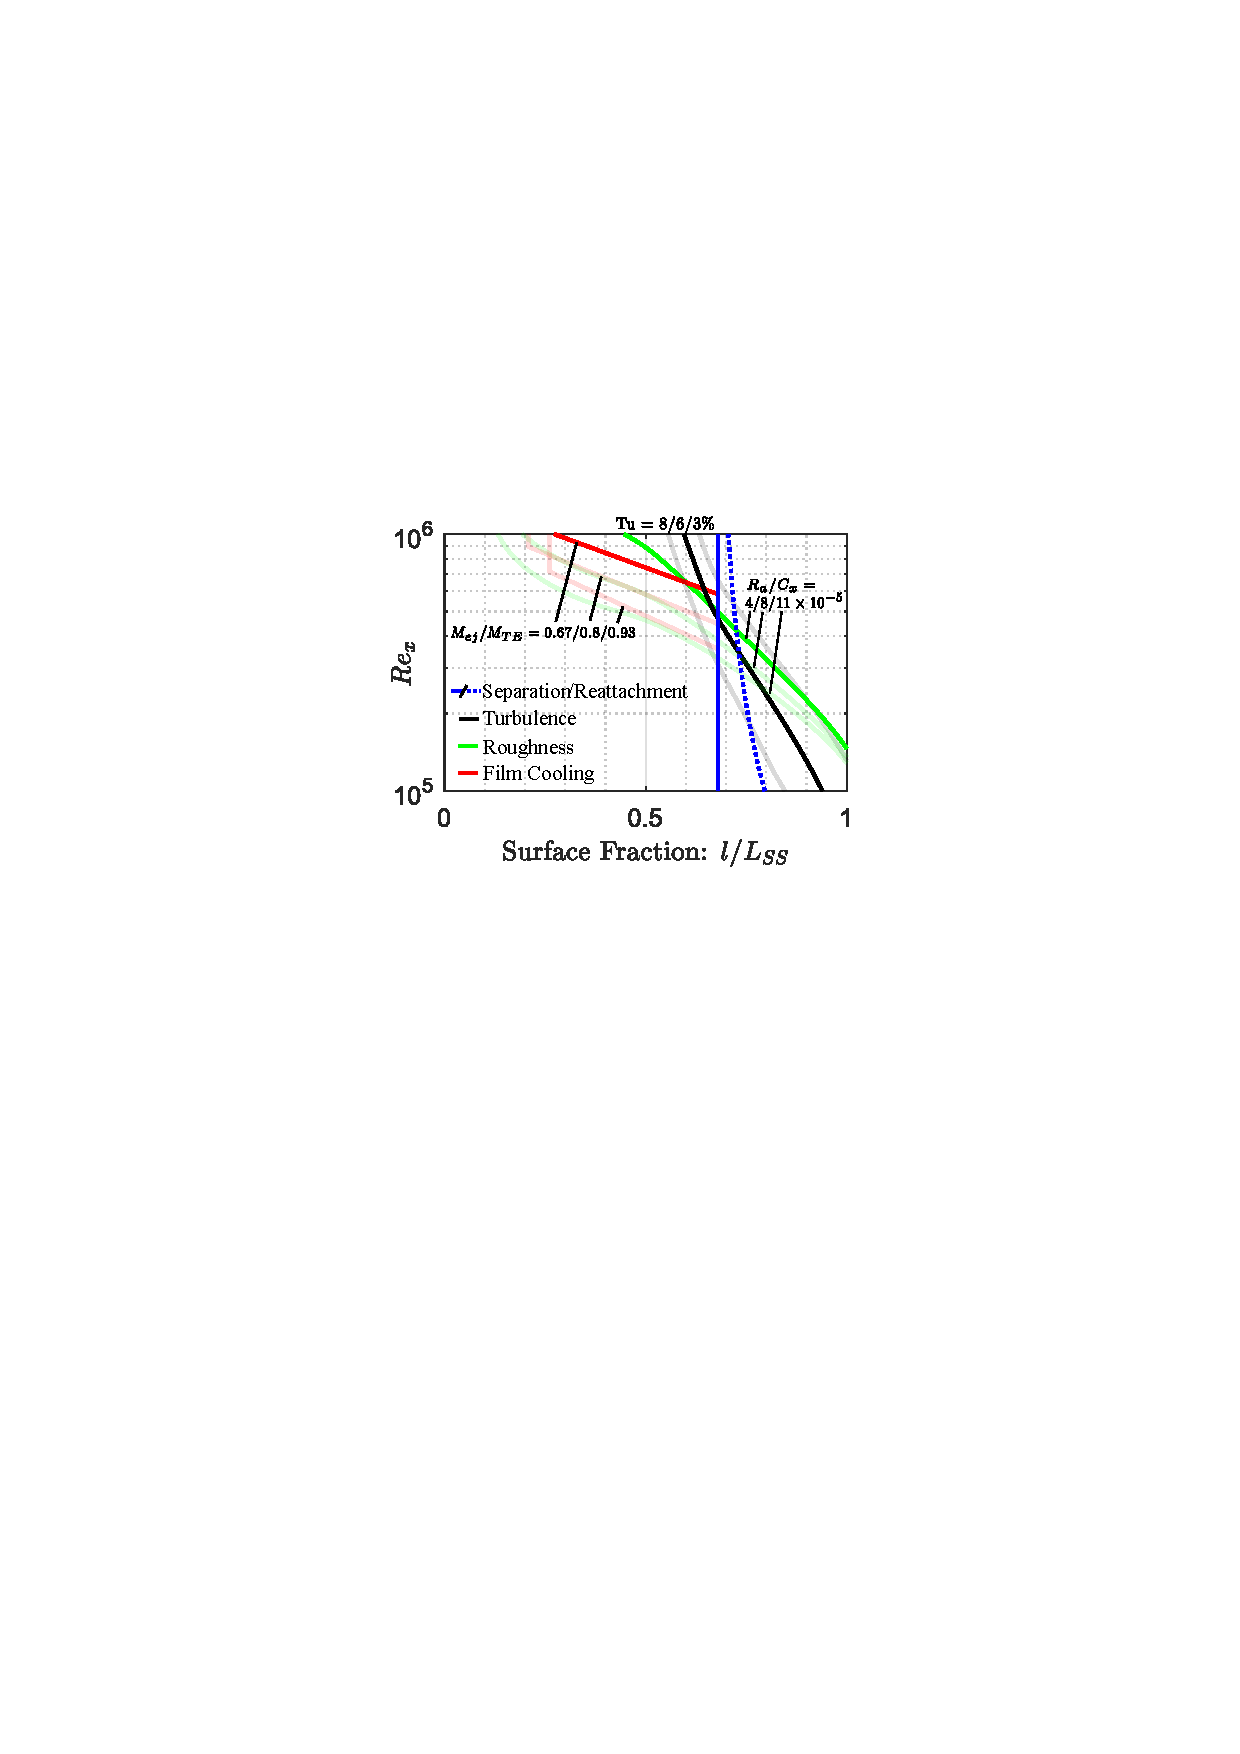
\includegraphics[width=0.5\textwidth]{fig_transition_map.pdf}
\caption{F1 (\texttt{figures/code/fig\_transition\_map.py}): primary transition mechanism on the HPT suction
surface against $\mathrm{Re}_x$, from Kar et al.\ (2026), reproduced there from Clark et al.\ (2024).}
\end{figure}

\textbf{P8 The present study.}
\begin{itemize}
\item The justification chain in one place: the RANS errors of P4 are known by place but not by share (P4);
  at VR near 1 the mixing is mostly broadband turbulence, the part E1 and E2 are written for, so the question is
  how much of the mixing each mechanism carries (P5); scale-resolving simulations give the reference, at a
  resolution not yet established (P6); the 7-7-7 is the most documented
  shaped hole (P2); a flat plate at zero pressure gradient fixes geometry and pressure gradient (P3); a laminar
  approach layer is relevant to small cores and hardest for RANS (P7). Together they make a test bed in which
  only the model and the mesh change.
\item The approach: one mesh family from 5M to 193M cells; steady RANS, LES and DNS; the same boundary conditions
  and plenum pressure on every rung.
\item Closing sentence leads into Section 2, the research aims.
\end{itemize}

%=====================================================================================================
\section*{2\quad Research Aims}
\textbf{Purpose.} A short section between the Introduction and the Methods, as in the GPPS paper: one framing
sentence (``This paper aims to \dots''), then the aims as a numbered list, one sentence each. No figures, tables
or equations.
\begin{enumerate}[label=\arabic*.]
\item Quantify the $\bar\eta$ error of each rung, RANS to 100M 3DNS, against the 193M reference.
\item Establish the resolution each mesh achieves and the resolution needed to predict $\bar\eta$.
\item Locate where and explain why the modelled turbulence departs from the resolved turbulence, through the
  assumptions of E1 and E2.
\item Identify which of these departures matter for $\bar\eta$.
\end{enumerate}
Wording of the aims is set with the Results plan; the conclusions mirror them.

%=====================================================================================================
\setcounter{figure}{1}
\setcounter{table}{0}
\section*{3\quad Methods}

%-----------------------------------------------------------------------------------------------------
\subsection*{3.1\quad Simulation Configuration and Computational Methods}
\textbf{Purpose.} Define what is simulated, with which codes and models, under which boundary conditions, and
how the domain is divided for analysis. After this subsection the reader can place any rung name or region name
used later in the paper.

\textbf{(i) Geometry and operating point.}
\begin{itemize}
\item Baseline 7-7-7 laidback fan-shaped hole (Schroeder and Thole, 2014): $D=7.75$\,mm, $30^\circ$
  inclination, pitch $6D$; single hole, periodic in $y$; coolant fed at the metering inlet face, no plenum.
\item Flow conditions, justified by the transitional HP turbine (Clark et al., 2024; Kar et al., 2026): Blasius
  layer, $\mathrm{Re}_\theta=180$ at the hole, $M_\infty=0.25$, Tu 5.5\,\% with $L=0.43D$, $\mathrm{Re}_D=2408$;
  raised viscosity $\mu_\infty=2.5\times10^{-4}$\,Pa\,s; adiabatic walls.
\item BR 1.5 at DR 1.5: peak of $\bar\eta$ in the 7-7-7 database. Definitions of BR, DR, VR, $I$, $\eta$,
  $\bar\eta$, $D/U_\infty$, FT. All rungs share the plenum $p_{0,c}$, so BR is an output of each rung (T1).
\end{itemize}

\textbf{Equations in (i)} (from \texttt{01\_configuration.tex}; E3, E4 numbered there, E5 inline there).
\begin{equation}
\mathrm{Re}_D=\frac{\rho_\infty U_\infty D}{\mu_\infty}=\frac{0.9003\times86.28\times0.00775}{2.5\times10^{-4}}=2408,
\qquad \theta=0.075D
\tag{E3}
\end{equation}
Purpose: fixes the Reynolds number of the hole and the approach layer, and justifies the raised viscosity
($\sim$14 times that of air) needed to reach it at the physical hole size and $M_\infty=0.25$.
\begin{equation}
\mathrm{BR}=\frac{\dot m_c/A_m}{\rho_\infty U_\infty},\qquad A_m=\frac{\pi D^2}{4},\qquad
\mathrm{DR}=\frac{\rho_c}{\rho_\infty},\qquad
\mathrm{VR}=\frac{\mathrm{BR}}{\mathrm{DR}},\qquad I=\frac{\mathrm{BR}^2}{\mathrm{DR}}
\tag{E4}
\end{equation}
Purpose: defines the operating point as the experiment does, so BR 1.5, DR 1.5 compares directly with the
7-7-7 database; $A_m$ is the metering cross-section.
\begin{equation}
\eta=\frac{T_{0,\infty}-T_w}{T_{0,\infty}-T_{0,c}},\qquad
\bar\eta(x)=\frac{1}{P}\int_{-P/2}^{P/2}\eta\,\mathrm{d}y,\qquad P=6D
\tag{E5}
\end{equation}
Purpose: adiabatic effectiveness and its pitch average, the performance measure used throughout the Results.
Numbered in the paper, since the Results refer to it. $\eta$ is reserved for the effectiveness; the Kolmogorov
length is $\eta_K$ (E8).

Not given as equations: $D/U_\infty=89.8$\,\textmu s and $1\,\mathrm{FT}=40D/U_\infty=3.59$\,ms (inline), and
Sutherland's law in 3DNS (named and cited, no formula).

\textbf{(ii) Computational methods.}
\begin{itemize}
\item One mesh family, one set of boundary conditions, one reference (193M 3DNS). RANS against 50M 3DNS on the
  same mesh isolates modelling; 50M, 100M and 193M 3DNS isolate resolution; the 20M LES differs in both (T1).
\item STAR-CCM+ RANS: coupled density-based solver, SST $k$--$\omega$ with $\gamma$--$\mathrm{Re}_\theta$, which
  keeps the approach layer laminar ($\mathrm{Re}_\theta=176$, $H=2.51$--2.64 at $x/D=-4$); max $y^+=1.1$;
  residuals down 6--8 decades. RANS on the 5M and 50M meshes agree to 0.06\,\% in BR. URANS returns the
  steady state and is not a rung.
\item Every rung, including the RANS, runs at the same plenum $p_{0,c}$. BR matching is not mentioned in the
  Methods: the need for it is introduced in the Results, where the differences in diffuser-bubble behaviour
  between rungs are described.
\item 3DNS: high-order compressible finite-difference code (Wheeler et al.); 7-point DRP stencil (1\,\% phase
  error at $\sim$4 points per wavelength; Tam and Webb, 1993); 8th-order filter, $sf=0.05$ on 50M (implicit
  LES), 0.03 on 100M and 193M; 20M LES with WALE.
\item Initialisation, flush (BR drift below 1\,\% over 0.5\,FT) and averaging time.
\end{itemize}

\textbf{Table T1: rungs and meshes} \st{draft}. One row per mesh of the family, with its scale factor and the
rungs run on it. Purpose: the single reference for every rung name and every mesh; $s$ links it to the
coarsening in 3.2. No machine or rank information.

\begin{table}[H]
\centering\footnotesize\setlength{\tabcolsep}{4pt}
\begin{tabular}{@{}l c c l l l c c@{}}
\toprule
mesh & $s$ & cells & solver & model & filter $sf$ & BR & averaging \\
\midrule
5M   & 0.30$^a$ & $5.77\times10^{6}$ & STAR-CCM+ & RANS, SST + $\gamma$--Re$_\theta$ & -- & 1.591 & steady \\
20M  & 0.453 & $2.31\times10^{7}$ & 3DNS & LES, WALE & 0.03 & 1.498 & 6\,FT \\
50M  & 0.628 & $5.31\times10^{7}$ & STAR-CCM+ & RANS, SST + $\gamma$--Re$_\theta$ & -- & 1.592 & steady \\
     &       &                    & 3DNS & none (implicit LES) & 0.05 & 1.516 & 6\,FT \\
100M & 0.796 & $1.13\times10^{8}$ & 3DNS & none & 0.03 & 1.526 & 6\,FT \\
193M & 1     & $1.92\times10^{8}$ & 3DNS & none (reference) & 0.03 & 1.521 & 10\,FT \\
\bottomrule
\end{tabular}
\caption{Draft of T1. $s$: scale factor of E6 (3.2). Cells: summed over the 23 blocks of each CGNS file in
\texttt{/mnt/Elements/DNS/meshes/}. BR: coolant mass flow through the diffuser sections at the common plenum
$p_{0,c}$, from \texttt{analysis/hole\_discharge/README.md}. Averaging: 193M batch b010.
$^a$\,The 5M mesh has the blocks of the family, but its counts were not set by E6; 0.30 is the average of
$(N_{5}-1)/(N_{193}-1)$ over the blocks, weighted by the 193M points in each block (per-line range 0.20--0.46).}
\end{table}

\textbf{(iii) Boundary conditions.} The same for every rung, so stated once, in text only (no table, no
separate figure; F2(a) marks where each applies):
\begin{itemize}
\item Inlet: Blasius layer, $\mathrm{Re}_\theta$ 135--140, with FST of Tu 5.5\,\%; outlet and top at
  $p_\infty$; adiabatic no-slip walls; periodic span; coolant inlet at the same $p_{0,c}$ and $T_{0,c}$ for
  every rung, with coolant turbulence.
\item How each code imposes them, in one sentence each: FST box and characteristic boundaries with buffers in
  3DNS, inlet intensity in STAR-CCM+; Sutherland viscosity in 3DNS, constant in STAR-CCM+.
\end{itemize}

\textbf{(iv) Analysis regions.} Eight regions that fill the domain without overlap (buffers excluded):
metering, diffuser (split $3.5D$ along the axis from the breakout), exit (breakout face extruded $0.5D$ each
way), approach layer, jet ($x/D$ $-1.00$ to 2.36), near film (to 10.25), far film (to 25), freestream
($z/D\ge4$). One sentence per boundary choice. Used in 3.3 and in every regional average of the Results.

\textbf{Figure F2: configuration, boundary conditions and regions} \st{draft}, full page width.
\begin{itemize}
\item Purpose: one picture for (i), (iii) and (iv). Panel (a) gives the domain extent, the hole position, the
  condition on every boundary and the five regions above the plate. Panel (b) enlarges the hole to show the
  metering, diffuser and exit regions and the coolant inlet face.
\item Every region is named on the figure; colour is not the only key. Okabe-Ito fills.
\item The 3DNS buffers are hatched, so ``excluded from all data'' has a visible meaning.
\item To finalise: hole outline from \texttt{cl\_outline.npy}; label sizes checked at the full page width of the
  ASME layout.
\end{itemize}
\begin{figure}[H]
\centering
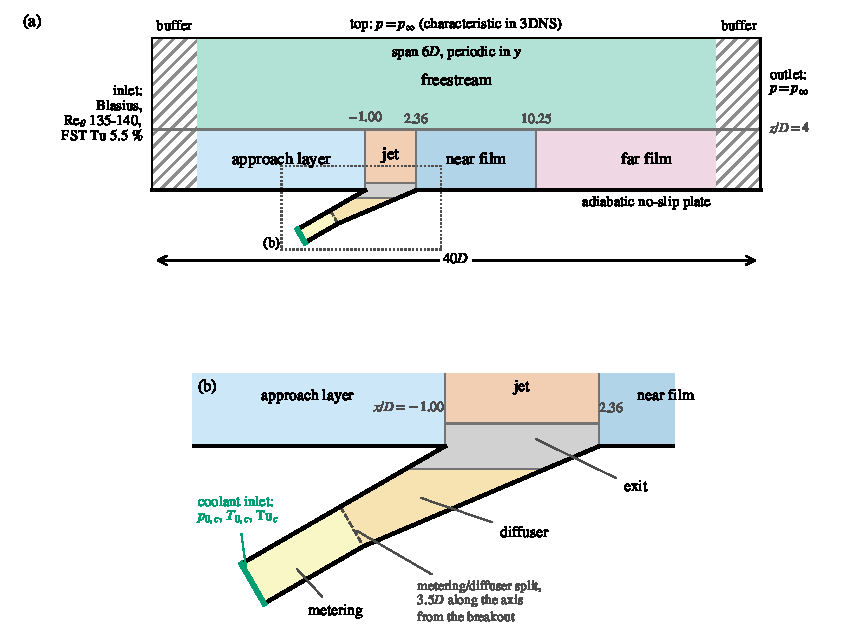
\includegraphics[width=0.92\textwidth]{fig_config_regions.pdf}
\caption{Draft of F2 (\texttt{figures/code/fig\_config\_regions.py}). (a) Centre plane of the domain, to scale,
with the boundary conditions and the regions above the plate. (b) Enlarged view of the hole with the hole
regions. Hatched: 3DNS buffer zones.}
\end{figure}

%-----------------------------------------------------------------------------------------------------
\subsection*{3.2\quad Mesh Family and Coarsening Method}
\textbf{Purpose.} Show that the meshes differ in resolution only: same blocks, walls and hole geometry,
obtained by coarsening the 193M mesh line by line.

\textbf{Content} (from \texttt{03\_mesh\_resolution.tex}; the decisions in \texttt{HANDOFF.md} are kept).
\begin{itemize}
\item The 193M mesh: 23 blocks; 80--100\,\um\ across the jet; 220--290\,\um\ axially in the hole; 40\,\um\ first
  cell; 1\,\% growth to $z/D=10$.
\item Coarsening: 13 classes of connected grid lines, one count per class; E6 with the $s$ of T1;
  points evenly spaced in 193M point number (E7), so the 193M stretching is kept and each cell grows by
  $\sim1/s$; wall cell kept; interface jumps below $\sim$1.5; cubic placement on the 193M line.
\item Departures from E6: classes 1, 9, 11 held at the 100M count; 2, 7, 8, 10 raised for load balance.
\item The 5M mesh shares the 23 blocks but was not built with E6; its representative $s$ is given in T1 and the
  range of its per-line ratios in the text.
\end{itemize}

\textbf{Equations} (from \texttt{03\_mesh\_resolution.tex}, both numbered there).
\begin{equation}
N=\operatorname{round}\!\big((N_{193}-1)\,s\big)+1,\qquad \text{cells}\approx s^3\times1.92\times10^{8}
\tag{E6}
\end{equation}
Purpose: the point count of every class on a coarser mesh from its 193M count $N_{193}$ and the one scale
factor $s$ of that mesh (T1); the second part links $s$ to the mesh size.
\begin{equation}
\xi_m=m\,\frac{N_{193}-1}{N-1},\qquad m=0,\dots,N-1
\tag{E7}
\end{equation}
Purpose: where the $N$ points of a coarser line sit, as fractional 193M point numbers $\xi$; even spacing in
$\xi$ keeps the 193M stretching and cell aspect ratios. The wall-cell and interface exceptions are stated in the
text, not as equations.

\textbf{Figure F3: the 13 line classes} \st{draft}.
\begin{itemize}
\item Purpose: makes ``class'' concrete; E6 and the class numbers quoted in the text refer to it.
\item Drawn to the figure rules: (a)/(b) labels in place of titles; Okabe-Ito colours with a line style per
  direction (solid $i$, dashed $j$, dash-dot $k$).
\item To finalise: class numbers are small at print size.
\end{itemize}
\begin{figure}[H]
\centering
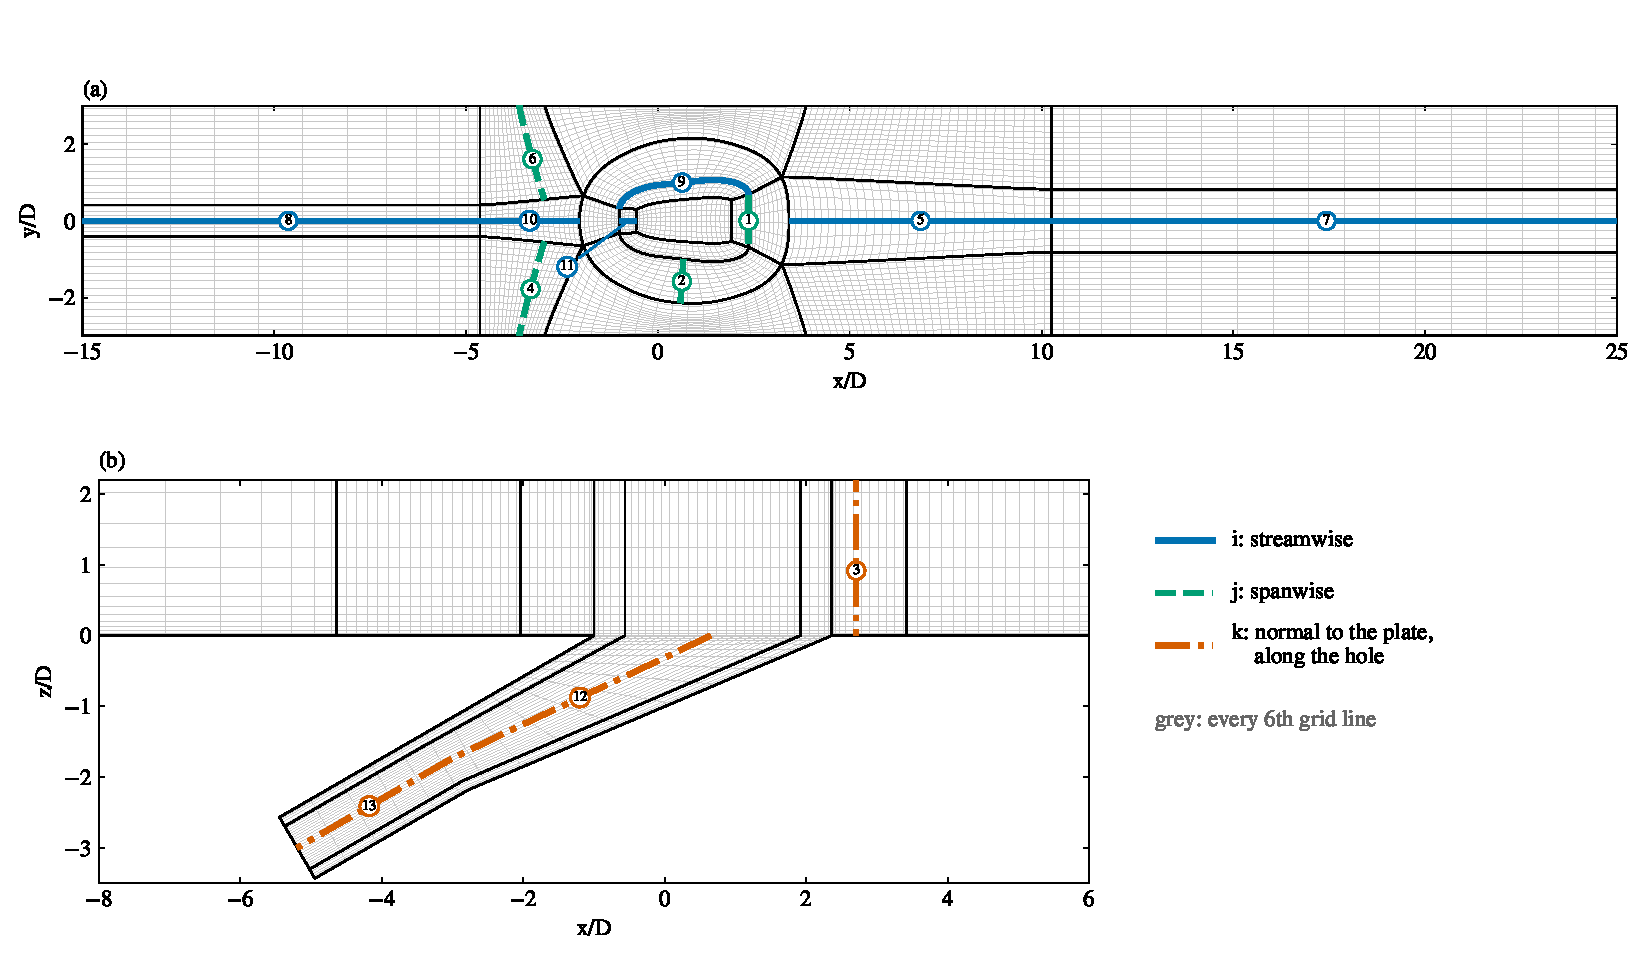
\includegraphics[width=0.85\textwidth]{fig_mesh_classes.pdf}
\caption{Draft of F3 (\texttt{figures/code/fig\_mesh\_classes.py}, 20M mesh). (a) Plate plane, all 23 blocks.
(b) Centre plane through the hole.}
\end{figure}

\textbf{In text, no table} (replaces the class table of \texttt{03\_mesh\_resolution.tex}):
\begin{itemize}
\item the classes that depart from E6 and why, by class number on F3: 1, 9, 11 held at the 100M counts across
  the hole (88, 215, 48 points); 2, 7, 8, 10 raised for load balance;
\item the 5M mesh: same blocks, per-line ratios $(N_5-1)/(N_{193}-1)$ of 0.20--0.46;
\item the cell sizes that stay fixed or bounded: first cell 40\,\um\ at the plate and 22\,\um\ in the hole on
  every mesh, cell-size jump across block interfaces below $\sim$1.5;
\item the 193M cell sizes (80--100\,\um\ across the jet, 220--290\,\um\ axially in the hole, 0.59\,mm at the top),
  which grow by $\sim1/s$ on the coarser meshes.
\end{itemize}

%-----------------------------------------------------------------------------------------------------
\subsection*{3.3\quad Achieved Mesh Resolution}
\textbf{Purpose.} State, for each mesh and region, how the grid size compares with the smallest scale of the
reference flow.

\textbf{Equation} (from \texttt{03\_mesh\_resolution.tex}, changed to the single reference $\eta_K$).
\begin{equation}
\frac{\Delta_{\mathrm{mesh}}}{\eta_{K,193}}\le2,\qquad \Delta_{\mathrm{mesh}}=|J|^{1/3},\qquad
\eta_{K,193}=\Big(\frac{\nu^3}{\varepsilon/\bar\rho}\Big)^{1/4},\qquad
\varepsilon=\overline{\tau_{ij}\partial_ju_i}-\bar\tau_{ij}\,\partial_j\bar u_i
\tag{E8}
\end{equation}
with $|J|$ the cell volume of the 5M, 20M, 50M, 100M or 193M mesh, $\nu=\bar\mu/\bar\rho$, and $\varepsilon$ the
viscous dissipation of the fluctuations, all from the 193M 3DNS, statistics batch b010 (10\,FT).
Purpose: the resolution criterion and the one quantity reported in F4 and the text. The bound 2 follows from
$\kappa_{\max}\eta_K\ge1.5$ for spectral DNS (Pope, 2000), i.e.\ $\Delta/\eta_K\le\pi/1.5\approx2.1$; stated
inline, not numbered.
\begin{itemize}
\item One $\eta_K$ field for all meshes. The ratio measures each mesh against the scales of the reference flow,
  so differences between meshes come from the mesh alone. The 5M and 50M RANS meshes are rated on the same
  scale as the scale-resolving rungs.
\item The lower-bound caveat of the draft (filtered or modelled dissipation on the 20M LES and 50M 3DNS) no
  longer applies, and no LES statistics are needed for the 20M mesh.
\item To state: $\eta_{K,193}$ is computed on the 193M mesh, so where the 193M is not resolved (diffuser) it is
  less certain.
\item Wall units: one sentence giving the maximum $y^+$, $x^+$ and $z^+$ on each mesh.
\item Convergence of the statistics between 100M and 193M is a separate criterion, referenced here.
\end{itemize}

\textbf{Method to compute it} (for the analysis agents). $\Delta_{\mathrm{mesh}}$ of each coarser mesh is mapped
onto the 193M points through the line-by-line correspondence of the family, and volume fractions are taken with
193M cell volumes, so every mesh uses the same region volumes. \texttt{dns/python/resolution\_regions.py} uses
each run's own $\varepsilon$ and is to be extended. The 5M mesh is mapped through its own per-line counts.

\textbf{In text, no table} (replaces the resolution table of \texttt{03\_mesh\_resolution.tex}):
\begin{itemize}
\item volume fraction with $\deta>2$ over the whole domain, per mesh;
\item the regions that are not resolved and by how much: diffuser, exit and far film on each mesh; the metering
  section in one sentence, since it is left out of F4;
\item $\eta_{K,193}$ in the diffuser ($\sim$47\,\um) against its 220--290\,\um\ axial cells, as the reason the
  diffuser is the least resolved region.
\end{itemize}
All numbers from the new computation (above); the draft values (batches b005/b006, own $\eta_K$, placeholder 20M)
are not used.

\textbf{Figure F4: volume distribution of $\deta$} \st{interim}. Fraction of each region's volume above a given
$\deta$, one line per mesh: 5M, 20M, 50M, 100M, 193M.
\begin{itemize}
\item Purpose: the main evidence of 3.3. Shows how far each mesh of the family sits from the criterion, region
  by region, from the RANS mesh to the reference, including the tails behind the values quoted in the text.
\item One row of panels: diffuser, exit, near film, far film and the whole domain. The metering section is
  left out of the figure and covered in one sentence of the text. Five meshes: Okabe-Ito colours with solid,
  dashed, dash-dot, dotted and one marker style.
\item The interim version below uses each run's own $\eta_K$ and the histogram regions $x/D$ 3--10 and 10--25.
  The final version uses $\eta_{K,193}$ for every mesh, adds the 5M curve and uses the region bounds of F2.
\end{itemize}
\begin{figure}[H]
\centering
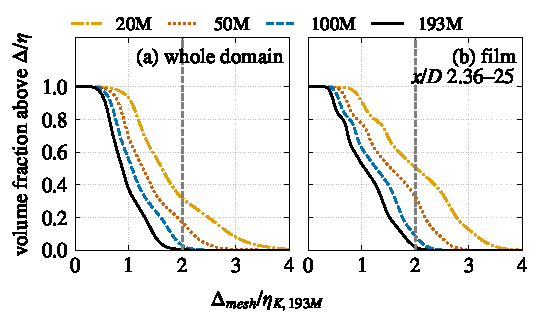
\includegraphics[width=\textwidth]{fig_resolution.pdf}
\caption{Interim F4 (\texttt{figures/code/fig\_resolution.py}): each run with its own $\eta_K$. Batches: 20M
LES b006, 50M 3DNS b006, 100M 3DNS b006 (6\,FT each), 193M 3DNS b010 (10\,FT). Dashed vertical line: ratio 2.}
\end{figure}

%=====================================================================================================
\section*{4\quad Results}
\textbf{Purpose.} The Results move from what the reader can see to what the closure does. Section 4.1 gives
the lay of the land: the coolant flow from the plenum to the film, the mainstream from the approach layer to the
far film, and the effectiveness they produce. Section 4.2 breaks the mean mixing of each rung down into its
causes and compares them with the literature. Section 4.3 (a posteriori tests) is planned once the tests are
done.

\textbf{Common to 4.1 and 4.2.}
\begin{itemize}
\item Rungs: the six of Section 3 only: RANS 5M and 50M, 20M LES, 50M, 100M and 193M 3DNS, all at the same
  plenum $p_{0,c}$. No corrected RANS (QCR, $\Pr_t$ sweep, substitution) before 4.3.
\item Reference: the 193M 3DNS at batch b010 (10\,FT), the record it was run for, in every figure and number.
  The lower rungs keep their last batch (b006, 6\,FT); the record-length check (193M b006 against b010: regional
  values move by 0.046 or less) is one sentence.
\item Quantities the reader knows are shown beside the new ones: $k/U_\infty^2$, shape factor $H$, $C_f$,
  $\mathrm{Re}_\theta$, intermittency $\gamma$, $k$ production $P_k$ and dissipation $\varepsilon$ (normalised by
  $U_\infty^3/D$), the dissipation length $k^{3/2}/\varepsilon$, the discharge coefficient $C_D$ and the static
  pressure along the hole. All 3DNS values come from the stat3 files (means, Favre stresses, heat fluxes,
  $\widetilde{T''^2}$, dissipation, pressure--dilatation, scalar dissipation); RANS values from the STAR cell
  exports.
\item Line plots in PDF, fields in PNG; $\eta$ and temperature fields in \texttt{jet}, other sequential fields in
  \texttt{inferno}, signed fields and log ratios in \texttt{bwr} with symmetric limits.
\end{itemize}

%-----------------------------------------------------------------------------------------------------
\subsection*{4.1\quad Coolant Flow}
\textbf{Purpose.} Lay of the land. Two chains of cause, each with flow-field figures, then the effectiveness
that both produce, then the frame in which the rest of the paper attributes the differences. About 2.5 pages.

\textbf{(i) First chain: from the plenum face through the hole.}
\begin{itemize}
\item The coolant enters at the plenum face at the same $p_{0,c}$ (81\,110\,Pa) on every rung, so BR is a
  result. It accelerates through the metering section and separates in the diffuser.
\item The diffuser separation depends on the modelling: the 3DNS hold two corner lobes on the downstream wall
  that grow from $s/D=-3.3$, peak at 16--19\,\% of the section near $s/D=-2.1$ and close at the exit; the RANS
  keeps two thin lobes of 9--10\,\%; the 20M LES lobes peak at 21\,\%.
\item The separation sets the pressure recovery of the diffuser, and through it the head across the metering
  section and the flow. The static rise from the metering section to the exit is 2627--2645\,Pa in the RANS
  against 1148--1554\,Pa in the scale-resolving rungs; the RANS also loses about 600\,Pa more in the metering
  section.
\item Result: BR 1.591--1.592 (RANS 5M and 50M, mesh-independent, so a model effect), 1.498 (20M LES), 1.516,
  1.526, 1.521 (50M, 100M, 193M 3DNS); the RANS passes 4.7\,\% more coolant, the 20M LES 1.5\,\% less. $C_D$ per
  rung in the text.
\item Literature: the diffuser recovery and the conical-diffuser analogy (Haydt et al., 2018); $C_D$ of
  expanded holes (Gritsch et al., 1998b); backflow at the 7-7-7 exit in iLES (Oliver et al., 2017). Not seen
  before: the rung-to-rung BR spread at one plenum pressure, traced to the diffuser recovery.
\item Bubble motion (193M b010, F7): the separated volume is $0.719\,D^3$ (50M 0.761; 10.9\,\% of the diffuser on
  the 50M) and varies by 10\,\% (standard deviation); the two lobes trade volume (correlation $-0.48$), with the
  volume spectrum peaking at St 0.078 and a second rise near St 0.27; BR is $1.527\pm0.019$ (1.2\,\%) and peaks
  at St 0.273, where it is coherent with the volume (0.78, 95\,\% level 0.21).
\item Effect on the mainstream (50M analysis, not yet repeated on the 193M): the slow mode at St 0.04 has 79\,\% of
  its energy in the film, but the lobe
  switching is not coherent with the film meander or the sideways shift of the cooled footprint (coherence
  $\le0.10$). Interpretation: the bubble motion modulates the coolant flow by about 1\,\% and does not organise
  the film. Consistent with Fawcett (2011) for VR near 1.
\item BR sensitivity in one sentence from the 7-7-7 data at DR 1.5: $\bar\eta$ ($x/D$ 7--15) 0.230, 0.243, 0.218
  at BR 1.0, 1.5, 2.0, so a 4.7\,\% BR difference moves $\bar\eta$ by much less than the RANS deficit of (iii).
\end{itemize}

\textbf{Figure F5: pressure and separation along the hole} \st{rework}. Two panels against $s/D$, six rungs:
(a) area-mean static pressure coefficient, (b) fraction of the section with reversed axial flow; metering and
diffuser marked.
\begin{itemize}
\item Purpose: shows in one view where the rungs part: the same metering drop for the scale-resolving rungs,
  a larger one for the RANS, and a diffuser recovery that follows the size of the reversed region.
\item Source: \texttt{analysis/hole\_discharge/plots.py} F3; redrawn to the figure rules, 5M RANS and 193M added.
\end{itemize}
\planfig{fig_hole_axis.pdf}{0.5}{F5 (\texttt{figures/code/fig\_hole\_axis.py}): (a) $C_{p,c}=(p-p_\infty)/(p_{0,c}-p_\infty)$,
(b) reversed-flow fraction of each section; all six rungs, 193M stat3 b010, other 3DNS and LES b006. 193M: BR
1.520, peak reversed fraction 0.159 at $s/D=-2.3$, diffuser static rise 1537\,Pa ($s/D$ $-4.9$ to $-0.9$); b006
within 0.1\,\% in BR and 7\,Pa in the rise. Complete.}

\textbf{Figure F6: mean flow in the diffuser} \st{rework}. Axial velocity $u_s/U_\infty$ on hole sections at
$s/D$ $-2.3$, $-1.1$ and $-0.5$ (rows), zero contour in black; RANS 50M, 20M LES, 193M 3DNS (columns; the 50M and
100M 3DNS in the text). The centre-plane reversed layer (0.03--0.07\,D thick) is given as numbers in the text.
\begin{itemize}
\item Purpose: the flow field behind F5: the thin RANS lobes against the thick corner lobes of the resolved
  rungs.
\item Format: PNG, \texttt{bwr} symmetric about zero. Source: \texttt{hole\_discharge} F4, F5.
\end{itemize}
\planfig{fig_diffuser_flow.png}{0.95}{F6 (\texttt{fig\_diffuser\_flow.py}): $\langle u_s\rangle/U_\infty$ on sections
$s/D=-2.3$ (a--c), $-1.1$ (d--f), $-0.5$ (g--i); $u_s=0$ line; colour range $\pm0.05$, forward flow saturates. 193M
b010, RANS 50M, 20M LES b006. Reversed area fraction (F5 values, cell-volume weighted): RANS 0.092, 0.089, 0.051;
20M LES 0.179, 0.148, 0.027; 193M 0.159, 0.100, 0.028. Text numbers, centre-plane layer: maximum thickness RANS
0.032\,D, 20M LES 0.072\,D, 193M 0.048\,D. Complete.}

\textbf{Figure F7: motion of the diffuser bubble} \st{new}. 193M 3DNS (b010 window): (a) time trace of the
separated volume $V$ (black) and of the volumes of the two corner lobes, $y>0$ and $y<0$ (orange and blue);
(b) spectra of $V$ and of BR; (c) coherence of $V$ with BR.
\begin{itemize}
\item Purpose: shows that the bubble moves (lobe exchange with a volume peak at St 0.078, pulsing near St 0.27)
  and how little of that reaches the coolant flow (BR varies by 1.2\,\%).
\item What the panels say, for the caption and the text:
  \begin{itemize}
  \item (a): the two lobes are the reversed-flow regions in the two lower corners of the diffuser (F6 (b)); when
    one grows the other shrinks (correlation $-0.48$; 50M $-0.59$), while their sum $V$ changes by only 10\,\%.
  \item (b): premultiplied spectra, $f\,\Phi(f)$ normalised by the variance, so equal areas mean equal shares of
    the variance; this shows where in frequency $V$ and BR fluctuate.
  \item (c): the magnitude-squared coherence $\gamma^2_{V,\mathrm{BR}}(f)$, between 0 and 1, is the share of
    the BR fluctuation at frequency $f$ that is linearly related to the bubble volume at the same frequency.
    The 95\,\% level is the value two unrelated signals would exceed by chance in only 5\,\% of cases, given the
    number of averaged segments ($1-0.05^{1/(n-1)}$ for $n$ independent segments); only coherence above it is
    taken as a real link. 193M: 0.78 at St 0.273, 0.39 at St 0.078, level 0.21 ($n=14$ segments of
    25.6\,$D/U_\infty$, 50\,\% overlap, inside the 13 gap-free stretches). 50M: 0.82, 0.35, level 0.24.
  \end{itemize}
\item Source: \texttt{hole\_discharge} W3 (b0, 381ca65; FINDINGS S15--S18): 1995 snapshots at 0.2\,$D/U_\infty$,
  99.97\,\% of the b010 window.
\end{itemize}
\planfig{fig_bubble_motion.pdf}{0.7}{F7 (\texttt{fig\_bubble\_motion.py}): (a) separated volume and the two lobe
volumes, (b) premultiplied spectra of the volume and BR, (c) their coherence with the 95\,\% level. 193M 3DNS,
b010 window (1995 snapshots). Complete.}

\textbf{(ii) Second chain: the mainstream.}
\begin{itemize}
\item The approach layer is laminar under decaying FST: at $x/D=-2.3$ the 3DNS give $H$ 2.58--2.62 (Blasius
  2.59), $\mathrm{Re}_\theta$ 175--182; the RANS gives $H$ 2.88 and $\mathrm{Re}_\theta$ 165. FST streaks raise
  $u_{rms}$ in the layer to 0.07--0.10\,$U_e$ in the 3DNS (Jacobs and Durbin, 2001; Brandt et al., 2004).
\item Behind the hole ($|y/D|\le1.5$) the jet trips the layer: the 3DNS layer is turbulent from $x/D\approx2$
  ($\gamma$ 0.93--1.00). The RANS layer behind the jet is turbulent too.
\item At mid-pitch the rungs part. In the 193M spots appear at $x/D$ 3--8 off the mid-pitch line and reach the
  line from $x/D$ 5--6; they stay small (0.5--1\,$D^2$), grow as they convect and merge into the downstream
  turbulent patch near $x/D\approx10$ (evidence: F9). Mid-pitch $\gamma$ is below 0.01 to $x/D=5$, 0.22 at
  $x/D=10$, 0.58 at 14, 0.89 at 20, first above 0.8 at $x/D=17$; $H$ falls to 1.71. The RANS mid-pitch layer stays
  laminar to $x/D=25$ ($\gamma\approx0.02$, $\mu_t/\mu\le0.6$, $H$ 2.2--2.6, $C_f$ $1.8$--$2.2\times10^{-3}$ against
  $2.4$--$5.6\times10^{-3}$).
\item Consequence: near-wall $k$ of the RANS between the jets is 0.02--0.14 of the 3DNS value, so there is no
  turbulent mixing to carry coolant to the mid-pitch.
\item Literature: holes trip a laminar layer (Goldstein and Yoshida, 1982); spot growth and merger in bypass
  transition (Zaki, 2013; Ovchinnikov et al., 2008); $\gamma$--$\mathrm{Re}_\theta$ has no film-cooling trip
  (Langtry and Menter, 2009).
\end{itemize}

\textbf{Figure F8: state of the wall layer} \st{rework}. Plan view of the plate ($x/D$ $-3$ to 25, one pitch),
near-wall $k/U_\infty^2$ at $z/D=0.1$ (top) and $\gamma$ (bottom); RANS 50M, 20M LES, 193M 3DNS.
\begin{itemize}
\item Purpose: the turbulent wedge behind each jet and the spread transition between the jets, against the
  laminar RANS mid-pitch.
\item Format: PNG, \texttt{inferno}. Source: \texttt{layer\_state} M1 ($\gamma$ maps); $k$ maps new from stat3
  and the cell exports.
\end{itemize}
\planfig{fig_wall_state.png}{0.95}{F8 (\texttt{fig\_wall\_state.py}): $k/U_\infty^2$ at $z/D=0.1$ (RANS 50M cell
layer, 20M LES b006, 193M b010) and $\gamma$ (RANS: model variable; 20M LES and 193M: own $z/D=0.1$ samplers,
threshold 0.0385\,$U_\infty^2/D$; own Otsu values 0.0374 and 0.0411). Mean $\gamma$ over the plate: RANS 0.17
(turbulent only behind the jet, about 0.02 between the jets), 20M LES 0.69, 193M 0.71. Complete.}

\textbf{Figure F9: spot growth and merger between the jets} \st{new}. 193M 3DNS (b010 window), plane sampler at
$z/D=0.1$: (a) space--time diagram of the turbulence indicator along the mid-pitch line, $x/D$ against
$tU_\infty/D$, with the Otsu threshold contour; (b) a sequence of 4--6 plan-view snapshots of the indicator at
fixed time steps, the same spot tracked from birth to merger.
\begin{itemize}
\item Purpose: the evidence for the spread transition: spots are born at $x/D$ 3--8 between the jets, grow as
  they convect and merge near $x/D\approx10$. In (a) a spot is a wedge whose leading and trailing edges give its
  celerities.
\item Numbers for the text (193M b010): leading- and trailing-edge celerities 0.46 and 0.40\,$U_\infty$ (median of
  18 spots; 50M 0.48 and 0.38), against about 0.9 and 0.5 in bypass transition (Zaki, 2013). Interpretation
  (medium confidence): a cut at $z/D=0.1$ under-reads the edge speeds, and the wedge is narrow. Tracked spot: born
  at $x/D=2.7$, 0.58\,$D^2$ at merger at $x/D=9.5$, 9.8\,$D/U_\infty$ later. Birth rate at most 2.5 per $D^2$ per
  100\,$D/U_\infty$ (upper bound). $\gamma_{\mathrm{mid}}(x)$ as in (ii).
\item Format: PNG, \texttt{inferno}. Source: new, from \texttt{layer\_state} (Otsu detector) applied to the 193M
  $z/D=0.1$ sampler.
\end{itemize}
\planfig{fig_spots.png}{0.95}{F9 (\texttt{fig\_spots.py}): spot growth and merger between the jets, 193M $z/D=0.1$
sampler, b010 window (3992 records, 400\,$D/U_\infty$); snapshots at $tU_\infty/D$ 282--292 of one spot from birth
($x/D=2.7$) to merger ($x/D=9.5$). Complete.}

\textbf{Figure F10: boundary-layer parameters along the plate} \st{new}. $H$ (a) and $C_f$ (b) against $x/D$ on the
centreline and at mid-pitch, six rungs; Blasius and turbulent correlations as references.
\begin{itemize}
\item Purpose: puts the transition of F8 into the parameters the reader knows, and shows where each rung
  departs.
\item Source: stat3 means and RANS exports (approach-layer values in \texttt{setup\_differences}, SU3, SU7;
  plate values in \texttt{layer\_state}, LS3).
\end{itemize}
\planfig{fig_bl_params.pdf}{0.8}{F10 (\texttt{fig\_bl\_params.py}): $H$ (a, b) and $C_f$ (c, d), centreline and mid-pitch, six rungs
(193M stat3 b010, others b006; RANS \texttt{bl\_summary.csv}); grey: Blasius and turbulent correlations. The 20M
LES spike at $x/D$ 19.8--20 is its outlet. Complete.}

\textbf{Figure F11: wall-normal profiles at $x/D=10$} \st{rework}. $U/U_\infty$, $k/U_\infty^2$ and $\gamma$
against $z/D$ on the centreline, at $y/D=1.5$ and at mid-pitch; RANS 50M, 20M LES, 193M 3DNS.
\begin{itemize}
\item Purpose: shows that the RANS difference sits through the whole layer at mid-pitch, not only at the wall.
\item Source: \texttt{layer\_state} L5, L6; extended to the 20M LES and 193M.
\end{itemize}
\planfig{fig_bl_profiles.pdf}{0.8}{F11 (\texttt{fig\_bl\_profiles.py}): $U/U_\infty$, $k/U_\infty^2$, $\gamma$ at
$x/D=10$ on the centreline, $y/D=1.5$ and mid-pitch; RANS 50M, 20M LES (b006), 193M (b010); $\gamma$ of the 20M
LES and 193M from their own $x/D=10$ planes (mid-pitch $\gamma$ at $z/D=0.1$: 0.26 and 0.20). Complete.}

\textbf{(iii) The outcome: effectiveness.}
\begin{itemize}
\item $\bar\eta$ over $x/D$ 2.5--7 / 7--15 / 15--20: RANS 0.270--0.272 / 0.168--0.171 / 0.138 (mesh-independent);
  20M LES 0.301 / 0.231 / 0.202; 50M 0.305 / 0.240 / 0.209; 100M 0.307 / 0.239 / 0.211; 193M (b010) 0.304 /
  0.237 / 0.208; experiment at Tu 0.5\,\% 0.293 / 0.243 / 0.212. The scale-resolving rungs agree within 0.008; the RANS is
  29--33\,\% low beyond $x/D=7$.
\item Centreline against mid-pitch: the RANS centreline is too high ($\eta$ 0.494 against 0.383 for the 193M at
  $x/D=20$), its mid-pitch too low (0.005--0.014 against the 193M 0.026 at $x/D=20$ and 0.043 at 25; experiment
  0.033--0.042).
\item Both chains feed this: the first sets the jet (BR, lift-off near the hole); the second sets the lateral
  mixing (a laminar RANS mid-pitch carries no coolant across the pitch). The RANS film is too narrow, not too
  weak.
\item The 3DNS mid-pitch $\eta$ is below the experiment (193M 0.004, 0.007, 0.015, 0.025 at $x/D$ 5, 10, 15,
  20 against 0.037, 0.033, 0.033, 0.035), although $\bar\eta$ agrees. Two explanations, both supported, neither
  alone sufficient:
  \begin{itemize}
  \item The approach layer differs. The experiment trips its layer at $x/D=-35$: turbulent, $H$ 1.45,
    $\mathrm{Re}_\theta$ 670 at $x/D=-4.7$ (Schroeder and Thole, 2014). The 3DNS layer is laminar, $H\approx2.6$,
    $\mathrm{Re}_\theta\approx180$. A turbulent layer mixes coolant to the mid-pitch from the hole on (the
    measured mid-pitch $\eta$ is flat at 0.033--0.037 from $x/D=2$).
  \item Transition takes distance. Tested on the 193M: $\eta_{\mathrm{mid}}$ is flat at 0.004--0.007 to
    $x/D=9$ and rises with $\gamma_{\mathrm{mid}}$; the gap narrows from $-0.033$ at $x/D=5$ to $-0.010$ at
    $x/D=20$. Where $\gamma_{\mathrm{mid}}>0.8$ ($x/D$ 17--20.5) the 3DNS is still 0.012 below (0.022 against
    0.034), so a fully turbulent mid-pitch does not close the gap: the coolant that a turbulent approach layer
    carries across from the hole on is missing upstream.
  \end{itemize}
  So the gap belongs to the laminar approach layer of the configuration (transition delay plus the missing
  upstream lateral mixing), not to a model or resolution error: all scale-resolving rungs agree (mid-pitch
  $\eta$ at $x/D=20$ 0.025--0.029). F12 (c) carries $\gamma_{\mathrm{mid}}(x)$ on a secondary axis.
\end{itemize}

\textbf{Figure F12: effectiveness against $x/D$} \st{rework}. (a) $\bar\eta$, (b) centreline $\eta$, (c)
mid-pitch $\eta$; six rungs and the 7-7-7 data at DR 1.5, BR 1.5.
\begin{itemize}
\item Purpose: the result the paper explains: the scale-resolving rungs on the data, the RANS low in $\bar\eta$,
  high on the centreline and near zero at mid-pitch.
\item Source: \texttt{validation\_50M} V1; 100M and 193M from \texttt{validation\_dns}; centreline and mid-pitch
  panels new.
\end{itemize}
\planfig{fig_eta_x.pdf}{0.55}{F12 (\texttt{fig\_eta\_x.py}): (a) $\bar\eta$, (b) centreline $\eta$, (c) mid-pitch $\eta$
($|y/D|=2.91$) with the 193M $\gamma_{\mathrm{mid}}$ (dashed grey, secondary axis); 193M b010, other rungs b006,
experiment id727 (DR 1.5, BR 1.5, Tu 0.5\,\%). Complete.}

\textbf{Figure F13: effectiveness on the wall} \st{new}. $\eta$ on the plate, $x/D$ 0--25, one pitch; RANS 50M,
20M LES, 193M 3DNS.
\begin{itemize}
\item Purpose: the narrow RANS footprint against the wide resolved one; links F8 (wall state) to F12.
\item Format: PNG, \texttt{jet}.
\end{itemize}
\planfig{fig_eta_wall.png}{0.75}{F13 (\texttt{fig\_eta\_wall.py}): $\eta$ on the plate, (a) RANS 50M, (b) 20M LES, (c)
193M 3DNS (b010; others b006); the exit footprint is blank (no plate faces there). Complete.}

\textbf{(iv) From the flow to the closure.}
\begin{itemize}
\item The coolant reaches the wall through the turbulent stress and heat flux of the mean equations. To attribute
  the $\eta$ differences to the flow, the two inputs of the RANS heat flux are measured in the reference: the
  eddy viscosity, as an effective eddy viscosity $\mu_{\mathrm{eff}}$ (E9), and the turbulent Prandtl number in
  its classic form (E10). The RANS heat flux is $c_p\mu_t/\Pr_t\,\nabla\tilde T$ (E2), so it is wrong if either
  input is wrong.
\item For the RANS they equal $\mu_t$ and 0.9 by construction (E1, E2); for the 3DNS they are measured from the
  stat3 stresses and fluxes. 4.2 breaks the $\mu_t$ difference down and compares the $\Pr_t$.
\item Owner decision (2026-11-25b): no effective diffusivity $\alpha_{\mathrm{eff}}$ and no tensor form of $\Pr_t$
  anywhere in the paper; one linear story.
\end{itemize}
\begin{equation}
\mu_{\mathrm{eff}}=-\frac{a\!:\!S^{*}}{2|S^{*}|^2},\qquad a^{\perp}=a+2\mu_{\mathrm{eff}}S^{*},\qquad a^{\perp}\!:\!S^{*}=0
\tag{E9}
\end{equation}
Purpose: the eddy viscosity that best fits the measured anisotropy $a$ to the mean strain $S^{*}$; $a^\perp$ is
the part no eddy viscosity can carry.
\begin{equation}
\Pr_t=\frac{\widetilde{u''w''}\big/\partial\tilde u/\partial z}{\widetilde{w''T''}\big/\partial\tilde T/\partial z},\qquad
\Pr_{t,R}=\frac{\sum_R\widetilde{u''w''}\,\partial_z\tilde u\big/\sum_R(\partial_z\tilde u)^2}
{\sum_R\widetilde{w''T''}\,\partial_z\tilde T\big/\sum_R(\partial_z\tilde T)^2}
\tag{E10}
\end{equation}
Purpose: the $\Pr_t$ of the paper, the quantity E2 sets to 0.9, in the form of Kohli and Bogard (2005); the
regional value $\Pr_{t,R}$ is the gradient-weighted least-squares fit, so low-gradient points carry little weight
and no point thresholds are needed; quoted for $z/D\ge0.3$, since the gradient weighting lets the viscous wall
layer dominate otherwise.

\textbf{Figure F14: turbulent Prandtl number of the reference} \st{rework}. Classic $\Pr_t$ (E10) of the 193M
3DNS on the centre plane and on the cross-plane $x/D=10$ (there also the lateral form), 0.9 marked on the colour
bar, dashed line where both gradients exceed the thresholds; candidate \texttt{fig\_prt\_classic.png}.
\begin{itemize}
\item Purpose: first look at the closure: in the film the reference mixes heat faster than momentum where E2
  assumes 0.9; near the wall compare with Kohli and Bogard ($\approx2$). Opens 4.2.
\item Near-wall values ($z/D<0.3$) only with their b006--b010 convergence: there $\widetilde{w''T''}$ and
  $\partial\tilde T/\partial z$ both tend to zero at the adiabatic wall.
\end{itemize}
\planfig{fig_prt_classic.png}{0.9}{F14 (\texttt{fig\_prt\_classic.py}): classic $\Pr_t$ (E10) of the 193M b010
(mean over 10\,FT), no masking, dashed line at the gradient thresholds: (a) centre plane; (b) near-wall strip,
$z/D$ 0--0.3, stretched; (c) $x/D=10$, wall-normal form (median 0.72 above thresholds); (d) $x/D=10$, lateral form
(0.65); (e) $x$-averaged least-squares $\Pr_t$ against $z/D$, near and far film, b010 with 95\,\% band and b006
dashed, RANS 0.9, Kohli and Bogard $\approx2$ (low FST) and $\approx1$ (high FST). Near-wall: 1.0--1.3 at
$z/D=0.1$, 0.5--0.7 from $z/D=0.2$; above 1.5 only at $z/D$ 0.04--0.08, not converged. Complete.}

%-----------------------------------------------------------------------------------------------------
\subsection*{4.2\quad Breakdown of Model Differences}
\textbf{Purpose.} One linear story (owner, 2026-11-25b). The RANS heat flux is $c_p\mu_t/\Pr_t\,\nabla\tilde T$
(E2), so it has two inputs. (1) $\mu_t$ is too low in the film, and the split of E13 shows why: mainly the
length scale of the mixing motions is too small; the energy is close and the alignment the RANS assumes is close
to the reference in the film (F18). (2) The heat flux inherits that, and the $\Pr_t$ setting of 0.9 is too high:
the reference classic $\Pr_t$ is $\sim$0.45 in the jet, near the free-shear value, and 0.6--0.8 in the film
(Kays, 1994; Schlichting and Gersten, 2017). (3) Spanwise: the reference mixes more laterally than wall-normally,
which an isotropic $\mu_t$ cannot represent (F20). Each point is compared with the literature; what is new is the
split and the assigned causes. Ends on the remedies, which lead into 4.3. About 3 pages.

\textbf{(i) The momentum factors and the log budget.}
\begin{itemize}
\item $\mu_{\mathrm{eff}}$ is the product of how much turbulence there is ($k^{1/2}$), the size of the motions
  that mix ($L_{\mathrm{eff}}$) and how well the stress lines up with the strain ($\cos\theta$) (E11).
\item The log of a ratio of products is a sum, so the difference between a rung and the reference splits
  exactly into the three factors (E12), and so does its average per region (E13), with no covariance term.
\item The energy factor ties to the familiar $k$ budget (E14): production $2|S^*|b_\parallel$ against
  dissipation; the length factor ties to the dissipation length, since $L_{\mathrm{eff}}$ equals
  $C_\mu k^{3/2}/\varepsilon$ within $\ln0.1$ in the jet and film of the reference.
\item The RANS has $\cos\theta=1$ and $\Pr_t=0.9$ by construction; the split shows what that costs.
\end{itemize}
\begin{equation}
\mu_{\mathrm{eff}}=\bar\rho\,k^{1/2}\,L_{\mathrm{eff}}\cos\theta,\qquad L_{\mathrm{eff}}=\frac{k^{1/2}|b|}{|S^*|}
\tag{E11}
\end{equation}
\begin{equation}
\ln\frac{\mu_{\mathrm{eff}}}{\mu_{\mathrm{eff}}^{193}}=\ln\frac{\bar\rho}{\bar\rho^{193}}
+\underbrace{\tfrac12\ln\frac{k}{k^{193}}}_{\text{energy}}
+\underbrace{\ln\frac{L_{\mathrm{eff}}}{L_{\mathrm{eff}}^{193}}}_{\text{length}}
+\underbrace{\ln\frac{\cos\theta}{\cos\theta^{193}}}_{\text{alignment}}
\tag{E12}
\end{equation}
\begin{equation}
\langle\ln r_\mu\rangle_{R}=\langle\ln r_\rho\rangle_{R}+\tfrac12\langle\ln r_k\rangle_{R}+\langle\ln r_L\rangle_{R}
+\langle\ln r_{\cos}\rangle_{R},\qquad \langle f\rangle_R=\frac{1}{V_R}\int_R f\,\mathrm dV
\tag{E13}
\end{equation}
\begin{equation}
\mathrm D\ln k=2|S^*|\,b_\parallel-\tfrac23\tilde S_{kk}-\frac{\varepsilon}{\bar\rho k}+\mathcal T_k,\qquad b_\parallel=|b|\cos\theta
\tag{E14}
\end{equation}
Purpose of E11--E14: E11 names the three momentum factors; E12 and E13 make them additive per point and per
region, which is what F15 shows; E14 links the energy factor to production and dissipation.

\textbf{(ii) Region by region.}
\begin{itemize}
\item Order: jet ($x/D$ 0--3), near film (3--10), far film (10--25) in full; diffuser, exit and approach layer in
  one paragraph; metering section in one sentence.
\item Scale-resolving rungs in one sentence, as a bound: their $\ln\mu_{\mathrm{eff}}$ totals against the 193M
  lie within $\pm2$\,SE of zero in the jet and film (W1 item 3, 1 Dec). The RANS differences are an order larger.
\item \textbf{Step 1, $\mu_t$ (F15, F17, F18, F19).} RANS 50M against the 193M b010 (W1 item 1, due 27 Nov; old
  values against the 50M: jet $+0.32$, near film $-0.57$, far film $-0.77$). The length factor is the largest term
  and negative in the film: on the centre plane the median $\ln(L_{\mathrm{RANS}}/L_{193})$ is $-0.64$ (near film)
  and $-0.56$ (far film), so the RANS motions are about half the size. The alignment the RANS assumes
  ($\cos\theta=1$) is close to the reference in the film (median $\cos\theta$ 0.83, a term of
  $\ln(1/0.83)=+0.19$), so it offsets little; the energy term is small except in the far film at mid-pitch, where
  the RANS layer is laminar (4.1 (ii)). In the film the deficit is therefore a length-scale deficit. In the jet
  the alignment is poor ($\cos\theta$ 0.28--0.73) and the length close ($+0.04$), so there the error is in the
  stress form. F19 ties $L_{\mathrm{eff}}$ to the dissipation length $C_\mu k^{3/2}/\varepsilon$ (ratio 1.02--1.07 on
  the centreline): the RANS $\omega$ sets the length too small.
\item \textbf{Step 2, $\Pr_t$ (F14, F16).} The RANS heat flux $c_p\mu_t/0.9\,\nabla\tilde T$ carries the $\mu_t$
  deficit of step 1, divided by a $\Pr_t$ that is too high.
\item Origin of 0.9: the solver default (stated in the text, no citation), representative of the 0.85--0.9
  backed out of log-layer profiles of a flat-plate boundary layer (Kays, 1994); about 0.5 is the free-shear value
  (Schlichting and Gersten, 2017); Kohli and Bogard (2005) note most models assume $\Pr_t\approx1$.
\item The setting (193M b010, classic form, least squares over the full centre plane, $z/D\ge0.3$; b006 in
  brackets): jet 0.44 (0.42; 95\,\% 0.27--0.55), near film 0.63 (0.67; 0.57--0.73), far film 0.80 (0.80;
  0.78--0.82). Below 0.9 everywhere; lowest where the flow is a free shear layer. By $\eta$ band the mixing layer
  gives 0.43 / 0.69 / 0.76 (jet / near / far film).
\item Near the wall (classic form, $x$-averaged, F14 (e)): 1.0--1.3 at $z/D=0.1$, 0.5--0.6 from $z/D=0.2$ outward,
  b006 against b010 within about 10\,\%. Values above 1.5 only at $z/D$ 0.04--0.08 in the near film, where b006 and
  b010 differ: not converged. No converged $\Pr_t\approx2$ (high confidence).
\item Consequence: lowering $\Pr_t$ to the reference value corrects the heat flux for a given $\mu_t$, but not the
  $\mu_t$ deficit of step 1, and an isotropic $\mu_t$ cannot carry step 3.
\item \textbf{Step 3, spanwise (F20).} The reference diffuses more laterally than wall-normally; an isotropic
  $\mu_t$ cannot. Numbers: $\nu_y/\nu_z$ and $\alpha_y/\alpha_z$ of the 193M (W2, 2 Dec; $x/D=10$ cross-plane now
  from the $\Pr_t$ agent); old 50M values 1.5--2.1 and 1.4--1.5 in the jet and film, against 1.5--4 of Kaszeta and
  Simon (2000). Known in the literature as the RANS culprit (Acharya et al., 2001; Harrison and Bogard, 2008a); new
  here: the lateral deficit assigned to its causes (length, $\Pr_t$ setting, anisotropy).
\item RANS sweep link (STAR session, 2026-11-25; FINDINGS LP6, reference 193M b010): global $\Pr_t$ 0.5, 0.4,
  0.3 move the centreline $\eta$ at $x/D=20$ from 0.494 to 0.356 (193M 0.383) but $\bar\eta$ ($x/D$ 20--25)
  saturates at 0.146--0.150 (193M 0.194); QCR gives 0.170, QCR with $\Pr_t$ 0.4 0.177. A $\Pr_t$ setting fixes the
  centreline, not the lateral spread; QCR alone raises the centreline (0.520). Recovered share of the $x/D$ 7--20
  $\bar\eta$ deficit against the 193M: $\Pr_t$ 0.5 / 0.4 / 0.3 alone 36 / 44 / 48\,\%; QCR alone 72\,\%; QCR with
  $\Pr_t$ 0.4 97\,\%; local $\Pr_t$ (0.4 near the hole, 0.9 beyond $x/D\approx10$) 34\,\%, with QCR 96\,\%. The
  stress form is worth more than the $\Pr_t$ setting. Mid-pitch $\eta$ at $x/D=20$ stays 0.006--0.012 in every
  run (193M 0.026). Leads to 4.3, which adds two runs approved on 2026-11-25: P1, zonal
  $\Pr_t$ (0.4 for $x/D\ge3$, 0.9 in the jet and hole), and P2, heat-flux substitution in the film only; both
  50M SST, start by 28 Nov. The laminar RANS mid-pitch is tested by RC-S9 (approved 2026-11-20): $\gamma=1$ for
  $x>0$, $z>0$, approach layer and hole unchanged; 5M: $\eta_{\mathrm{plate}}$ $+1.3$\,\%, 50M smoke $+1.26$\,\%;
  50M production ends about 26 Nov.
\item Kohli and Bogard (2005): $\Pr_t\approx2$ at low freestream turbulence (0.6\,\%, a factor 4 variation) and
  $\approx1$, nearly uniform, at high (20\,\%). The 193M freestream $Tu$ is 3.3--3.6\,\% ($x/D$ $-5$ and 0,
  $z/D$ 2--3), between the two. The present near-wall 1.0--1.3 at $z/D=0.1$ falling to 0.5--0.6 sits nearer their
  high-turbulence value; their geometry (round holes, DR 1.05) also differs.
\item Volume values of the classic $\Pr_{t,R}$ from W1 item 4 (27 Nov) replace the plane values.
\item What the mixing motions are: the periodic (coherent) share of $\mu_{\mathrm{eff}}$ is 0.06--0.12 in the
  hole, jet and film (method of Lav et al., 2019); the mixing is mostly broadband turbulence, as Fawcett (2011)
  predicts at VR near 1, and the RANS gets the size of these motions wrong.
\item Alignment in the reference: mean strain builds the aligned anisotropy and mean rotation removes 55--114\,\%
  of it; a linear eddy viscosity keeps the strain drive only (budgets of $b_\parallel$, $b_\perp$).
\item Literature at each point: SST $\nu_t$ too low in the film (Stratton and Shih, 2019); non-uniform,
  anisotropic diffusivity (Kaszeta and Simon, 2000, ratio 1.5--4; Coletti et al., 2013); low and varying $\Pr_t$
  (Ling et al., 2016; Liu et al., 2008, 2011; Milani et al., 2019); Kohli and Bogard (2005) as above; lateral
  temperature spread under-predicted with $\Pr_t=0.9$ in a planar jet, by about 20\,\% (Rochhausen et al., 2015).
  For each: agrees or not, in one clause.
\end{itemize}

\textbf{Figure F15: why the RANS $\mu_t$ is low} \st{rework}. One panel: stacked bars of the energy, length and
alignment terms of $\ln(\mu_t/\mu_{\mathrm{eff}}^{193})$ with the total as a marker, RANS 50M against the 193M b010
only, per region (jet, near film, far film; diffuser, exit, approach layer narrower).
\begin{itemize}
\item Purpose: the main evidence of step 1: the length term carries the film deficit; the alignment term is small
  in the film and large in the jet. No scale-resolving bars (owner, 2026-11-25b): their bound is one sentence.
\item Values on the bars, $\pm2$ jackknife SE on the totals. Source: W1 item 1,
  \texttt{analysis/meff\_rans50\_c193b10/results\_pp/regions\_se.txt}, due 27 Nov.
\end{itemize}
\planfig{fig_meff_split.pdf}{0.95}{F15 (\texttt{fig\_meff\_split.py}), old layout (interim, against the 50M and
with scale-resolving panels); redrawn to one RANS 50M panel when W1 item 1 lands (27 Nov).}

\textbf{Figure F16: $\Pr_t$ of the reference against the setting and the literature} \st{new}. One panel: classic
$\Pr_{t,R}$ (E10) of the 193M b010 for $z/D\ge0.3$ in the jet, near film and far film (centre plane) and on the
$x/D=10$ cross-plane, b006 hollow, 95\,\% bars; lines at the RANS 0.9, the log-layer 0.85 (Kays, 1994), the
free-shear 0.5 (Schlichting and Gersten, 2017; Rochhausen et al., 2015) and Kohli and Bogard (2005), $\approx1$
and $\approx2$.
\begin{itemize}
\item Purpose: step 2 in one view: the setting is too high everywhere, by most in the jet, where the reference sits
  near the free-shear value.
\item Source: $\Pr_t$ analysis (\texttt{fig\_prt\_regions.py}, being drawn); volume values from W1 item 4.
\end{itemize}
\planfig{fig_prt_regions.pdf}{0.6}{F16 (\texttt{fig\_prt\_regions.py}): classic regional $\Pr_t$ of the 193M against
the setting and the literature; being drawn.}

\textbf{Figure F17: the mixing motions on cross-planes} \st{new}. $y$--$z$ planes at $x/D$ 4, 10 and 20:
$k/U_\infty^2$ (top) and $L_{\mathrm{eff}}/D$ (bottom), RANS 50M against 193M 3DNS, with $\eta$ contour lines.
\begin{itemize}
\item Purpose: the flow field behind F15: where the RANS has less turbulence (mid-pitch, far film) and where its
  motions are too small (jet and film edges), next to where the coolant sits.
\item Format: PNG, \texttt{inferno}.
\end{itemize}
\planfig{fig_cross_planes.png}{0.95}{F17 (\texttt{fig\_cross\_planes.py}): $k/U_\infty^2$ (a--f) and $L_{\mathrm{eff}}/D$
(g--l), RANS 50M and 193M 3DNS (b010), $x/D$ 4, 10, 20; white: $\eta$ 0.1--0.4. No masking: every point is drawn.
$L_{\mathrm{eff}}/D$ on a log scale, 0.01--1. In the freestream $|S^*|\to0$, so $L_{\mathrm{eff}}=k^{1/2}|b|/|S^*|$
of the 3DNS is patchy, 0.05--1 (j--l); the RANS length there is uniform, set by its freestream $k$ and $\omega$. 193M medians: $k/U_\infty^2$ $1.4\times10^{-3}$, $1.3\times10^{-3}$,
$2.4\times10^{-3}$, and $L_{\mathrm{eff}}/D$ 0.07, 0.10, 0.14 over the strained points (0.15, 0.14, 0.16 over all
points) at $x/D$ 4, 10, 20. Complete.}

\textbf{Figure F18: length and alignment on the centre plane} \st{rework}. $\ln(L_{\mathrm{eff}}/L_{\mathrm{eff}}^{193})$
of the RANS 50M (top) and $\cos\theta$ of the 193M 3DNS (bottom), $x/D$ $-2$ to 25.
\begin{itemize}
\item Purpose: locates the terms of F15 in the flow, length first: (a) the RANS length is short over the whole
  film; (b) in the film the reference is close to aligned (red, $\cos\theta\approx0.8$), so the RANS assumption
  $\cos\theta=1$ holds there and the length is the factor; misalignment only in the jet, near the wall and in the
  hole.
\item Format: PNG, \texttt{bwr}, symmetric limits. Source: \texttt{meff\_*} F2.
\end{itemize}
\planfig{fig_centre_factors.png}{0.9}{F18 (\texttt{fig\_centre\_factors.py}): centre plane, (a)
$\ln(L_{\mathrm{RANS}}/L_{193})$, (b) $\cos\theta$ of the 193M 3DNS (b010). No masking; blank only the wall row
($k=0$). Medians, points above the $|S^*|$ threshold / all points: $\ln$ ratio $+0.04/+0.22$ (jet), $-0.64/-0.35$
(near film), $-0.56/-0.42$ (far film); $\cos\theta$ 0.73/0.31, 0.83/0.71, 0.83/0.80; $\cos\theta<0$ at 18\,\% of
points. Complete.}

\textbf{Figure F19: turbulence budget and lengths along wall-normal lines} \st{new}. Centreline and mid-pitch at
$x/D$ 4, 10, 20: (a) $P_k$ and $\varepsilon$ in units of $U_\infty^3/D$; (b) $L_{\mathrm{eff}}$ against
$C_\mu k^{3/2}/\varepsilon$; RANS 50M, 20M LES, 193M 3DNS.
\begin{itemize}
\item Purpose: ties the energy and length factors to quantities the reader knows: where production sustains
  $k$, and that $L_{\mathrm{eff}}$ is the physical dissipation length in the film.
\item Source: \texttt{dns/python/tke\_budget\_pf.py} and \texttt{budgets\_c50b} B1, extended to the 193M.
\end{itemize}
\planfig{fig_budget_lines.pdf}{0.95}{F19 (\texttt{fig\_budget\_lines.py}): (a--c, d--f) $P_k$ (lines) and
$\varepsilon$ (markers) over $\rho_\infty U_\infty^3/D$, centreline and mid-pitch at $x/D$ 4, 10, 20; (g--i, j--l)
$L_{\mathrm{eff}}$ (lines) and $C_\mu k^{3/2}/\varepsilon$ (markers); 193M (b010), 50M and 20M LES (b006), RANS
50M. 193M medians over $z/D$ 0.05--1.5: $P_k/\varepsilon$ 1.27, 1.03, 0.90 (centreline) and 0.64, 1.57, 1.34
(mid-pitch); $L_{\mathrm{eff}}/(C_\mu k^{3/2}/\varepsilon)$ 1.02--1.07 (centreline), 0.74--1.22 (mid-pitch).
Complete.}

\textbf{Figure F20: spanwise diffusion} \st{rework}, simpler. (a) Lateral over wall-normal eddy diffusivity,
$\nu_y/\nu_z$ and $\alpha_y/\alpha_z$, per region of the 193M b010, with the band of Kaszeta and Simon (2000) and
the RANS value 1; (b) if the data allow, the lateral heat flux of the RANS 50M against the 193M at $x/D$ 4, 10, 20,
its deficit split into $\mu_t$, $\Pr_t$ setting and anisotropy.
\begin{itemize}
\item Purpose: step 3, one message: the reference agrees with the measured anisotropy (or not), and the new
  part is how much of the narrow RANS film each cause carries.
\item Source: $\Pr_t$ analysis ($x/D=10$ cross-plane, being drawn); W2 (2 Dec) for the regional values.
\end{itemize}
\planfig{fig_prt_data.pdf}{0.8}{F20 (\texttt{fig\_prt\_data.py}): old two-panel version (50M, 20M LES); being
redrawn on the 193M.}

\textbf{(iii) What the literature offers against each factor} (end of 4.2, leads to 4.3).
\begin{itemize}
\item Length scale: no film-cooling-specific correction of the SST length; data-driven eddy viscosity (Ling et
  al., 2016b; Milani et al., 2020).
\item $\Pr_t$ too high: lower or variable $\Pr_t$ (Liu et al., 2008, 2011; Lakehal, 2002); data-driven diffusivity
  (Milani et al., 2018, 2020; Ellis and Xia, 2024; Laroche et al., 2023; Qaragoez and Mazaheri, 2025).
\item Spanwise and alignment: anisotropic eddy viscosity (Azzi and Lakehal, 2002); quadratic constitutive relation
  (Spalart, 2000; Sabnis et al., 2021).
\item Energy in the far film: the transition model holds the mid-pitch laminar; no film-cooling trip exists in
  $\gamma$--$\mathrm{Re}_\theta$ (Langtry and Menter, 2009).
\item Each remedy targets one factor, while the split shows all three in error, the length the most. Closing
  sentence: Section 4.3 tests which remedy recovers $\bar\eta$ a posteriori.
\end{itemize}

%-----------------------------------------------------------------------------------------------------
\subsection*{4.3\quad A Posteriori Tests}
Planned once the tests are done.

\end{document}
